\usetikzlibrary{arrows.meta, positioning, calc, shapes.geometric, fit, patterns}

\tikzset{
  swbase/.style={draw, align=center, font=\footnotesize, inner sep=3pt,
                 line width=0.5pt,
                 execute at begin node={\hyphenpenalty=10000\relax\exhyphenpenalty=10000\relax}},
  swproc/.style={swbase, rectangle, minimum height=7mm, text width=#1},
  swproc/.default=34mm,
  swterm/.style={swbase, rectangle, rounded corners=3.4mm,
                 minimum height=7mm, text width=#1},
  swterm/.default=30mm,
  swdec/.style={swbase, diamond, aspect=2.4, inner sep=0.5pt, text width=#1},
  swdec/.default=24mm,
  % predefined process (detailed in another figure): box with side bars
  swsub/.style={swproc=#1, inner xsep=4.5mm,
    path picture={
      \draw[line width=0.5pt]
        ([xshift=1.6mm]path picture bounding box.north west) --
        ([xshift=1.6mm]path picture bounding box.south west)
        ([xshift=-1.6mm]path picture bounding box.north east) --
        ([xshift=-1.6mm]path picture bounding box.south east);}},
  swsub/.default=30mm,
  swarr/.style={-{Latex[length=2mm]}, line width=0.5pt},
  swdbl/.style={{Latex[length=2mm]}-{Latex[length=2mm]}, line width=0.5pt},
  swlbl/.style={font=\scriptsize, inner sep=1.5pt},
  swhw/.style={swbase, rectangle, minimum height=8mm, text width=#1,
               fill=black!10},
  swhw/.default=26mm,
}

\providecommand{\swtodo}[1]{\textbf{[TODO: #1]}}

\usetikzlibrary{arrows.meta, positioning, calc, shapes.geometric, fit, patterns}

\tikzset{
  swbase/.style={draw, align=center, font=\footnotesize, inner sep=3pt,
                 line width=0.5pt,
                 execute at begin node={\hyphenpenalty=10000\relax\exhyphenpenalty=10000\relax}},
  swproc/.style={swbase, rectangle, minimum height=7mm, text width=#1},
  swproc/.default=34mm,
  swterm/.style={swbase, rectangle, rounded corners=3.4mm,
                 minimum height=7mm, text width=#1},
  swterm/.default=30mm,
  swdec/.style={swbase, diamond, aspect=2.4, inner sep=0.5pt, text width=#1},
  swdec/.default=24mm,
  % predefined process (detailed in another figure): box with side bars
  swsub/.style={swproc=#1, inner xsep=4.5mm,
    path picture={
      \draw[line width=0.5pt]
        ([xshift=1.6mm]path picture bounding box.north west) --
        ([xshift=1.6mm]path picture bounding box.south west)
        ([xshift=-1.6mm]path picture bounding box.north east) --
        ([xshift=-1.6mm]path picture bounding box.south east);}},
  swsub/.default=30mm,
  swarr/.style={-{Latex[length=2mm]}, line width=0.5pt},
  swdbl/.style={{Latex[length=2mm]}-{Latex[length=2mm]}, line width=0.5pt},
  swlbl/.style={font=\scriptsize, inner sep=1.5pt},
  swhw/.style={swbase, rectangle, minimum height=8mm, text width=#1,
               fill=black!10},
  swhw/.default=26mm,
}

\chapter{Software Design}
\label{chap:software_design}

The hardware described in Chapter~\ref{chap:hardware_design} has the ability to apply a
potential to the cell and measure the current that flows, but it is the
firmware that turns these two features into a useful measurement.
This chapter describes the structure of the firmware and the logic of how a measurement is performed.

% The firmware has four tasks; to generate the DPV waveform, to sample and convert the cell current, to store the result, and to present it to the user.


\begin{figure}[H]
  \centering
  \caption{Software structure.
    Arrows show the direction of calls or data.}
  \label{fig:architecture}
  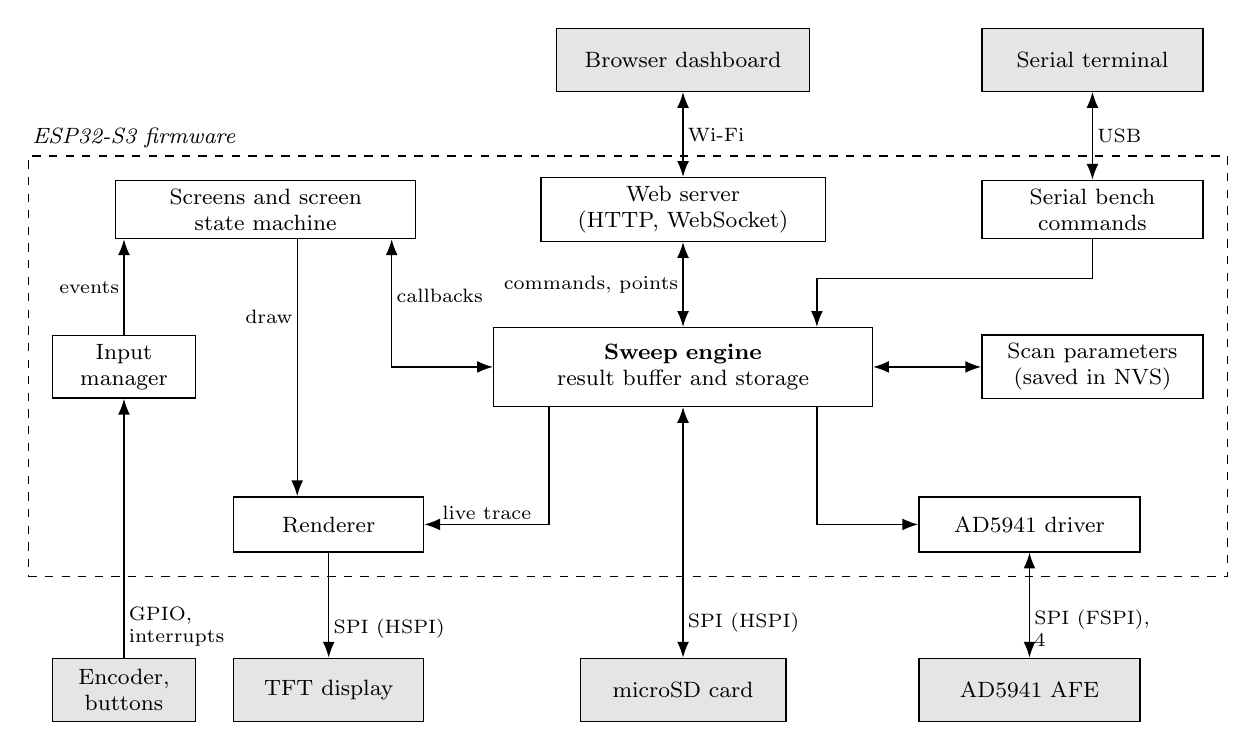
\begin{tikzpicture}[x=1cm, y=1cm]
    % --- external, top
    \node[swhw=30mm] (browser) at (7.6, 6.9) {Browser dashboard};
    \node[swhw=26mm] (pc)      at (12.8, 6.9) {Serial terminal};
    % --- row A
    \node[swproc=36mm] (screens) at (2.3, 5.0) {Screens and screen\\state machine};
    \node[swproc=34mm] (web)     at (7.6, 5.0) {Web server\\(HTTP, WebSocket)};
    \node[swproc=26mm] (serial)  at (12.8, 5.0) {Serial bench\\commands};
    % --- row B
    \node[swproc=16mm] (input)  at (0.5, 3.0) {Input\\manager};
    \node[swproc=46mm, minimum height=10mm] (engine) at (7.6, 3.0)
      {\textbf{Sweep engine}\\result buffer and storage};
    \node[swproc=26mm] (params) at (12.8, 3.0) {Scan parameters\\(saved in NVS)};
    % --- row C
    \node[swproc=22mm] (render) at (3.1, 1.0) {Renderer};
    \node[swproc=26mm] (driver) at (12.0, 1.0) {AD5941 driver};
    % --- firmware boundary
    \node[draw, dashed, line width=0.5pt, inner sep=3mm,
          fit=(screens)(serial)(input)(render)(driver)(params)] (fw) {};
    \node[swlbl, anchor=south west, font=\footnotesize\itshape]
      at ([yshift=0.3mm]fw.north west) {ESP32-S3 firmware};
    % --- hardware, bottom
    \node[swhw=16mm] (enc)  at (0.5, -1.1) {Encoder,\\buttons};
    \node[swhw=22mm] (tft)  at (3.1, -1.1) {TFT display};
    \node[swhw=24mm] (sd)   at (7.6, -1.1) {microSD card};
    \node[swhw=26mm] (afe)  at (12.0, -1.1) {AD5941 AFE};
    % --- connections
    \draw[swdbl] (browser) -- node[swlbl, right] {Wi-Fi} (web);
    \draw[swdbl] (pc) -- node[swlbl, right] {USB} (serial);
    \draw[swarr] (enc) -- node[swlbl, right, align=left, pos=0.12] {GPIO,\\interrupts} (input);
    \draw[swarr] (input.north) -- node[swlbl, left] {events}
      (input.north |- screens.south);
    \draw[swarr] ([xshift=-4mm]render.north |- screens.south) --
      node[swlbl, left, pos=0.3] {draw} ([xshift=-4mm]render.north);
    \draw[swdbl] ([xshift=16mm]screens.south) |-
      node[swlbl, right, pos=0.22] {callbacks} (engine.west);
    \draw[swarr] ([xshift=-17mm]engine.south) |-
      node[swlbl, above, pos=0.75] {live trace} (render.east);
    \draw[swdbl] (web) -- node[swlbl, left] {commands, points} (engine);
    \draw[swarr] (serial.south) -- ++(0,-0.5) -| ([xshift=17mm]engine.north);
    \draw[swdbl] (params) -- (engine);
    \draw[swarr] ([xshift=17mm]engine.south) |- (driver.west);
    \draw[swarr] (render) -- node[swlbl, right, pos=0.72] {SPI (HSPI)} (tft);
    \draw[swdbl] (engine) -- node[swlbl, right, pos=0.86] {SPI (HSPI)} (sd);
    \draw[swdbl] (driver) --
      node[swlbl, right, align=left, pos=0.72] {SPI (FSPI),\\\SI{4}{\mega\hertz}} (afe);
  \end{tikzpicture}
\end{figure}

Each of the modules in Figure~\ref{fig:architecture} is described in the sections that follow.

\section{Software Overview}
\label{sec:sw_overview}

The firmware is written in C++ on the Arduino framework for the ESP32-S3 and
is built with PlatformIO. Third-party libraries like Adafruit GFX and ST7735 are used for the display, ESPAsyncWebServer and AsyncTCP for
the web server and ArduinoJson for JSON encoding.


There were three design decisions shaped the structure of the software:
\begin{itemize}[label=\textbullet]
  \item \textbf{Project-specific AD5941 driver.} Analog Devices
    supplies a general-purpose software library for the AFE, which covers every measurement mode of the device. The driver for this project was adapted from this library and was written around the needs of this project. This gives
    the firmware direct control of the gain resistor $R_\text{TIA}$ of the
    transimpedance amplifier, which the automatic range selection in
    Section~\ref{sec:sw_ranging} switches repeatedly before a scan.

  \item \textbf{One sweep engine, two front ends.} The on-device screens and
    the web dashboard both start, stop and observe a measurement through the
    same sweep engine, so a scan behaves identically regardless of the interface that started the sweep.
  \item \textbf{A dedicated SPI bus for the AFE.} The display and the SD card
    share an SPI bus so
    display and storage traffic never occupies the bus used for the
    measurement.
\end{itemize}


% \begin{figure}[H]
%   \centering
%   \begin{tikzpicture}[x=1cm, y=1cm]
%     % --- external, top
%     \node[swhw=30mm] (browser) at (7.6, 6.9) {Browser dashboard};
%     \node[swhw=26mm] (pc)      at (12.8, 6.9) {Serial terminal};
%     % --- row A
%     \node[swproc=36mm] (screens) at (2.3, 5.0) {Screens and screen\\state machine};
%     \node[swproc=34mm] (web)     at (7.6, 5.0) {Web server\\(HTTP, WebSocket)};
%     \node[swproc=26mm] (serial)  at (12.8, 5.0) {Serial bench\\commands};
%     % --- row B
%     \node[swproc=16mm] (input)  at (0.5, 3.0) {Input\\manager};
%     \node[swproc=46mm, minimum height=10mm] (engine) at (7.6, 3.0)
%       {\textbf{Sweep engine}\\result buffer and storage};
%     \node[swproc=26mm] (params) at (12.8, 3.0) {Scan parameters\\(saved in NVS)};
%     % --- row C
%     \node[swproc=22mm] (render) at (3.1, 1.0) {Renderer};
%     \node[swproc=26mm] (driver) at (12.0, 1.0) {AD5941 driver};
%     % --- firmware boundary
%     \node[draw, dashed, line width=0.5pt, inner sep=3mm,
%           fit=(screens)(serial)(input)(render)(driver)(params)] (fw) {};
%     \node[swlbl, anchor=south west, font=\footnotesize\itshape]
%       at ([yshift=0.3mm]fw.north west) {ESP32-S3 firmware};
%     % --- hardware, bottom
%     \node[swhw=16mm] (enc)  at (0.5, -1.9) {Encoder,\\buttons};
%     \node[swhw=22mm] (tft)  at (3.1, -1.9) {TFT display};
%     \node[swhw=24mm] (sd)   at (7.6, -1.9) {microSD card};
%     \node[swhw=26mm] (afe)  at (12.0, -1.9) {AD5941 AFE};
%     % --- connections
%     \draw[swdbl] (browser) -- node[swlbl, right] {Wi-Fi} (web);
%     \draw[swdbl] (pc) -- node[swlbl, right] {USB} (serial);
%     \draw[swarr] (enc) -- node[swlbl, right, align=left, pos=0.2] {GPIO,\\interrupts} (input);
%     \draw[swarr] (input.north) -- node[swlbl, left] {events}
%       (input.north |- screens.south);
%     \draw[swarr] ([xshift=-4mm]render.north |- screens.south) --
%       node[swlbl, left, pos=0.3] {draw} ([xshift=-4mm]render.north);
%     \draw[swdbl] ([xshift=16mm]screens.south) |-
%       node[swlbl, right, pos=0.22] {callbacks} (engine.west);
%     \draw[swarr] ([xshift=-17mm]engine.south) |-
%       node[swlbl, above, pos=0.75] {live trace} (render.east);
%     \draw[swdbl] (web) -- node[swlbl, left] {commands, points} (engine);
%     \draw[swarr] (serial.south) -- ++(0,-0.5) -| ([xshift=17mm]engine.north);
%     \draw[swdbl] (params) -- (engine);
%     \draw[swarr] ([xshift=17mm]engine.south) |- (driver.west);
%     \draw[swarr] (render) -- node[swlbl, right, pos=0.72] {SPI (HSPI)} (tft);
%     \draw[swdbl] (engine) -- node[swlbl, right, pos=0.86] {SPI (HSPI)} (sd);
%     \draw[swdbl] (driver) --
%       node[swlbl, right, align=left, pos=0.72] {SPI (FSPI),\\\SI{4}{\mega\hertz}} (afe);
%   \end{tikzpicture}
%   \caption{Software architecture.
%     Arrows show the direction of calls or data.}
%   \label{fig:sw_architecture}
% \end{figure}

The dedicated bus keeps display and storage traffic away from the measurement
in hardware, but all of these modules still share the processor's time. How
that time is divided, and when the measurement takes priority, is set by the
top-level program flow.

\section{Top-Level Program Flow}  
\label{sec:sw_toplevel}

All project code runs from a single loop, shown in
Figure~\ref{fig:sw_toplevel}. During boot-up the device does a check to see if the WiFi, SD card  and AD5941 is working correctly, after these checks are done the user is taken into the home display. The state of the device is stored in three places, the active screen, a flag that records whether a scan is running, and the phase of the DPV step inside the AFE driver. The loop services each of these in turn on
every pass and none of them blocks the loop, except when the device is sampling which is discussed in Section~\ref{sec:sw_sampling}.

\begin{figure}[!htb]
  \centering
  \caption{Top-level program flow: start-up sequence (left) and the
    cooperative main loop (right).}
  \label{fig:sw_toplevel}
  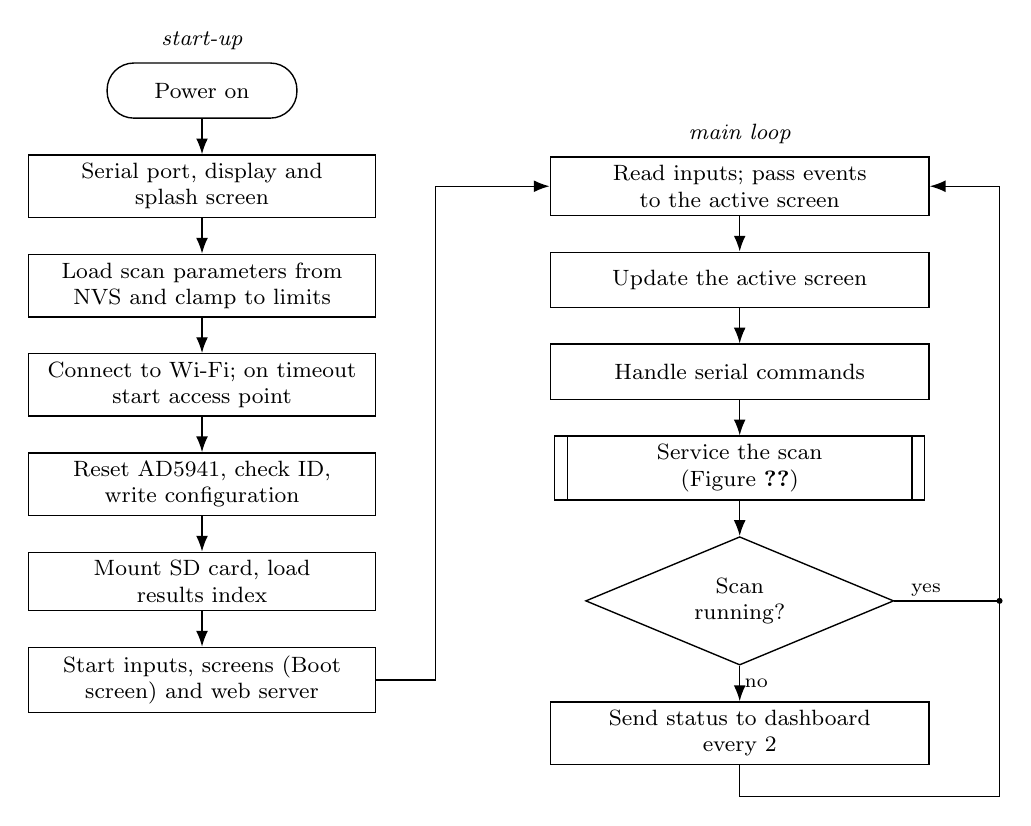
\begin{tikzpicture}[node distance=4.5mm and 12mm]
    % --- start-up column
    \node[swterm=22mm] (pwr) {Power on};
    \node[swproc=42mm, below=of pwr] (disp) {Serial port, display and\\splash screen};
    \node[swproc=42mm, below=of disp] (nvs) {Load scan parameters from\\NVS and clamp to limits};
    \node[swproc=42mm, below=of nvs] (wifi) {Connect to Wi-Fi; on timeout\\start access point};
    \node[swproc=42mm, below=of wifi] (afe) {Reset AD5941, check ID,\\write configuration};
    \node[swproc=42mm, below=of afe] (sd) {Mount SD card, load\\results index};
    \node[swproc=42mm, below=of sd] (ui) {Start inputs, screens (Boot\\screen) and web server};
    \foreach \a/\b in {pwr/disp, disp/nvs, nvs/wifi, wifi/afe, afe/sd, sd/ui}
      \draw[swarr] (\a) -- (\b);
    % --- loop column
    \node[swproc=46mm, right=22mm of disp] (l1) {Read inputs; pass events\\to the active screen};
    \node[swproc=46mm, below=of l1] (l2) {Update the active screen};
    \node[swproc=46mm, below=of l2] (l3) {Handle serial commands};
    \node[swsub=38mm, below=of l3] (l4) {Service the scan\\(Figure~\ref{fig:sw_scan})};
    \node[swdec=24mm, below=of l4] (l5) {Scan\\running?};
    \node[swproc=46mm, below=of l5] (l6) {Send status to dashboard\\every \SI{2}{\second}};
    \foreach \a/\b in {l1/l2, l2/l3, l3/l4, l4/l5}
      \draw[swarr] (\a) -- (\b);
    \draw[swarr] (l5) -- node[swlbl, right] {no} (l6);
    \coordinate (lb) at ($(l6.south)+(3.3,-0.4)$);
    \draw[swarr] (l6.south) -- ++(0,-0.4) -- (lb) |- (l1.east);
    \draw[line width=0.5pt] (l5.east) -- node[swlbl, above, pos=0.3] {yes} (l5.east -| lb);
    \fill (l5.east -| lb) circle (1.1pt);
    \draw[swarr] (ui.east) -- ++(0.75,0) |- (l1.west);
    \node[swlbl, anchor=south, font=\footnotesize\itshape] at ([yshift=1mm]l1.north) {main loop};
    \node[swlbl, anchor=south, font=\footnotesize\itshape] at ([yshift=1mm]pwr.north) {start-up};
  \end{tikzpicture}
\end{figure}

% ---------------------------------------------------------------------
\section{DPV Measurement Sequence}
\label{sec:sw_dpv}

A scan is defined by the parameters required in Table~\ref{tab:sw_params}. They are
stored in non-volatile storage (NVS), a partition of the ESP's flash memory, edited on the device and restricted to the limits seen in Table~\ref{tab:sw_ranges} whenever they are loaded or edited to protect the hardware. The scan rate is not set directly and is found by dividing the number of steps by the period.

\begin{table}[H]
  \centering
  \small
  \caption{DPV scan parameters, their default values and permitted ranges.}
  \label{tab:sw_params}
  \begin{tabular}{@{}llll@{}}
    \toprule
    \textbf{Parameter} & \textbf{Symbol} & \textbf{Default} & \textbf{Permitted range} \\
    \midrule
    Start potential   & $E_\text{start}$    & \SI{0.80}{\volt}        & \SI{-0.35}{\volt} to $E_\text{end} - \Delta E_\text{s}$ \\
    End potential     & $E_\text{end}$      & \SI{1.30}{\volt}        & $E_\text{start} + \Delta E_\text{s}$ to \SI{1.30}{\volt} \\
    Step              & $\Delta E_\text{s}$ & \SI{5}{\milli\volt}     & \SIrange{1}{50}{\milli\volt} \\
    Pulse amplitude   & $\Delta E_\text{p}$ & \SI{25}{\milli\volt}    & \SIrange{-100}{100}{\milli\volt} \\
    Pulse width       & $t_\text{p}$        & \SI{50}{\milli\second}  & \SIrange{10}{500}{\milli\second} \\
    Pulse period      & $T$                 & \SI{500}{\milli\second} & \SIrange{50}{5000}{\milli\second} \\
    TIA range         & $R_\text{TIA}$      & automatic               & automatic, or one of eight fixed values \\
    \bottomrule
  \end{tabular}
\end{table}

\subsection{Generating the Potential}
\label{sec:sw_potential}

The cell potential is set by the two outputs of the low-power DAC of the
AD5941. The 6-bit output $V_\text{ZERO}$ biases the high-speed transimpedance
amplifier (TIA), which holds the working electrode at that voltage, and is
fixed at \SI{1.7125}{\volt}. The 12-bit output $V_\text{BIAS}$ drives
the reference electrode through the potentiostat amplifier and carries the
staircase and the pulses. 

The applied potential is therefore
\begin{equation}
  E = V_\text{ZERO} - V_\text{BIAS}, where
  \qquad
  V_\text{BIAS} = \SI{0.2}{\volt} + D_{12}\times\frac{\SI{2.2}{\volt}}{4095},
  \label{eq:sw_potential}
\end{equation}
and $D_{12}$ is the 12-bit code and one code is \SI{537.2}{\micro\volt} which represents the voltage change per code. With
$V_\text{ZERO}$ fixed at this value, the permitted range of $E$ in
Table~\ref{tab:sw_params} keeps $V_\text{BIAS}$ between \SI{0.41}{\volt} and
\SI{2.06}{\volt}, inside the \SIrange{0.2}{2.4}{\volt} output range of the DAC.

\subsection{Scan Flow}

Before any timing starts, the TIA range is selected (Section~\ref{sec:sw_ranging}) and the requested timing is checked against the minimum that the sampling scheme can support
(Section~\ref{sec:sw_sampling}), a scan that fails this check is stopped. The scan consists of
\begin{equation}
  N = \left\lfloor \frac{E_\text{end} - E_\text{start}}{\Delta E_\text{s}} \right\rfloor
  \label{eq:sw_npoints}
\end{equation}
% CHECK: for the defaults this is 100 on paper, but the firmware evaluates it
% in single-precision floating point and (by the summary's arithmetic) gets
% 99. Confirm against the serial line "Sweep state: RUNNING (DPV, N points".
points, and the end potential itself is not applied as a base level. Each
point is produced by the step routine in Figure~\ref{fig:sw_step}, which the
main loop calls on every pass. The routine returns immediately unless a
sampling window is due, so the user interface stays responsive during the
\SI{450}{\milli\second} base dwell.

Points are held in memory during the scan and written to the SD card as a
single file only once the scan has stopped, so that card activity cannot
disturb the measurement. Every way of leaving a scan, whether completion, a
stop request or an overload, passes through the same stop routine, which stops
the ADC, returns the cell to $E = \SI{0}{\volt}$ and saves the points captured
so far. For more detail Figure~\ref{fig:sw_scan} in Appendix~\ref{app:scan_flow_timing} shows the process of how one scan is run. 


\section{Pulse Sampling and Timing}
\label{sec:sw_sampling}

DPV rejects the capacitive charging current only if $I_\text{before}$ and
$I_\text{end}$ are each sampled after the transient from the preceding edge
has decayed, as shown in Section~\ref{sec:dpv_rejection}. When the current is sampled, and for how long, therefore sets both
the noise of the measurement and how much charging current leaks into
$\Delta I$.

\subsection{Software Timing}
\label{sec:sw_timing}

All DAC updates and ADC conversions are done on the microcontroller. The staircase and the pulses are individual DAC writes over SPI, scheduled by the ESP32-S3 against its millisecond clock, and data-ready is detected by polling the interrupt flag register of the AD5941. This was a deliberate choice: timing the measurement in firmware gives the ESP32-S3 full control over when every operation in the system takes place, so the measurement can be scheduled around the display, storage and network activity instead of running alongside it.

That control is used to give the measurement priority over everything else
while a scan is running. Whenever the current is being sampled, the firmware
does nothing but sample: the buttons are not read, the display is not
updated and nothing is written to the SD card. This keeps the
digital activity of the device out of the sampling windows, which reduces the
noise coupled into the measurement and improves its accuracy. The cost is
that the timing between windows depends on the main loop, and the sampling
scheme below was designed so that this dependence does not reach the measured
current.

\subsection{Averaging Window}
\label{sec:sw_window}

The AD5941 has an analog path that has to be wide so that the cell current is converted faithfully as it changes at each pulse edge. The HSTIA is specified  for signals up to \SI{200}{\kilo\hertz} \cite[p.~50]{ad5941_ds}. Before the ADC of the AD5941 transmits the measurements to the ESP32-S3 its output
passes through two digital filters inside the device, a sinc3 filter
followed by a sinc2 filter \cite[p.~57]{ad5941_ds}. A sinc filter is a
low-pass filter that averages a block of consecutive samples and outputs
one result per block, so it both suppresses noise and lowers the data rate.
The number of samples per output is the oversampling ratio. In the
configuration used, the sinc3 filter reduces the raw \SI{800}{\kilo\hertz}
ADC rate by a factor of 5 to \SI{160}{\kilo\hertz}, and the sinc2 filter
reduces it further by a factor of 178 \cite[p.~59]{ad5941_ds}, resulting in an effective sampling frequency of \SI{900}{\hertz}. The digital bandwidths of the sinc3 filter is about \SI{42}{\kilo\hertz} and the sinc2 filter is \SI{290}{\hertz} The device also offers a
\SI{50}{\hertz}/\SI{60}{\hertz} notch filter after the sinc2 filter, but with
it enabled the settling time after a step is \SI{37}{\milli\second}, against
\SI{2.245}{\milli\second} without it \cite[p.~17]{ad5941_ds}. A
\SI{37}{\milli\second} settling time would consume most of a
\SI{50}{\milli\second} pulse, so the notch filter is bypassed and mains
rejection is provided in firmware instead: each current value is the mean of
$N_\text{w} = 18$ consecutive sinc2 results. The window length is
\begin{equation}
  T_\text{w} = N_\text{w} T_\text{s} = 18 \times \SI{1.1125}{\milli\second}
             = \SI{20.025}{\milli\second},
  \label{eq:sw_window}
\end{equation}
which is one period of the \SI{50}{\hertz} mains to within
\SI{0.13}{\percent}. This places zeros at multiples of 49.95Hz creating an effective filter. The window is defined by a sample count and not by a
duration, so every window in a scan has exactly the same length, and the ADC
runs continuously for the whole scan so that the filters are never restarted
between windows.

\subsection{Placing Windows}

Figure~\ref{fig:sw_timing} shows where the two windows fall within a step.
Each window starts \SI{21}{\milli\second} before the edge that follows it,
so that it ends at the edge: $I_\text{before}$ is the mean current over the
last \SI{20}{\milli\second} of the base dwell and $I_\text{end}$ the mean over
the last \SI{20}{\milli\second} of the pulse. These are the points of each
phase at which the charging current has had the longest time to decay.

\begin{figure}[!htb]
  \centering
  \caption{One DPV step with the default timing. Shaded bands show the two averaging windows.}
  \label{fig:sw_timing}
  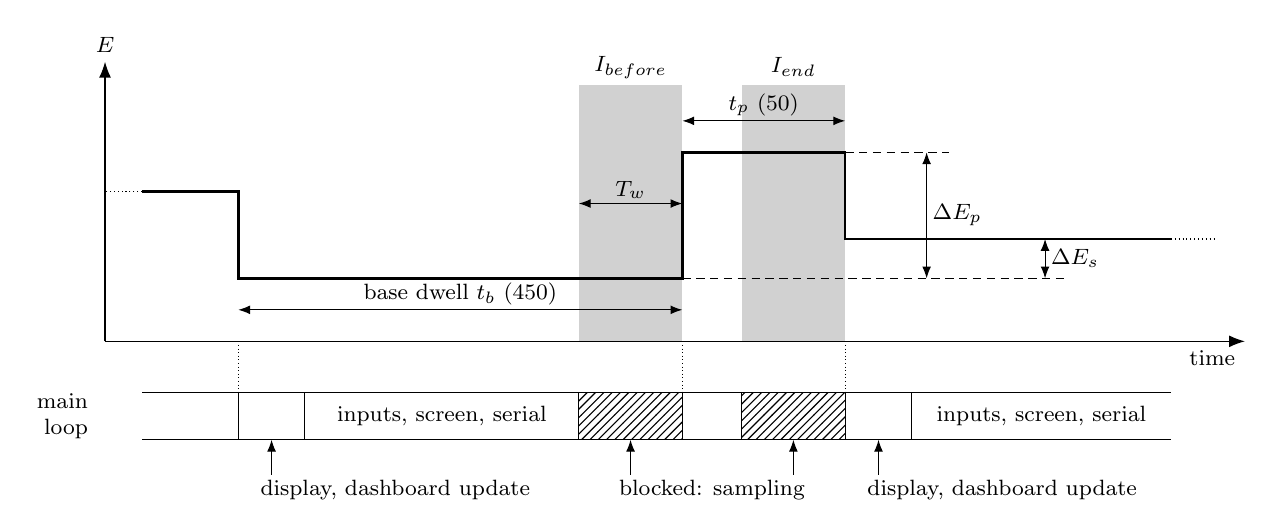
\begin{tikzpicture}[x=0.94cm, y=1cm, font=\footnotesize]
    % sampling windows
    \fill[black!18] (4.6,0.2) rectangle (6.0,3.45);
    \fill[black!18] (6.8,0.2) rectangle (8.2,3.45);
    \node[swlbl, font=\footnotesize] at (5.3,3.68) {$I_\text{before}$};
    \node[swlbl, font=\footnotesize] at (7.5,3.68) {$I_\text{end}$};
    % waveform
    \draw[line width=0.9pt]
      (-1.3,2.1) -- (0,2.1) -- (0,1.0) -- (6.0,1.0) -- (6.0,2.6) -- (8.2,2.6)
      -- (8.2,1.5) -- (12.6,1.5);
    \draw[densely dotted] (12.6,1.5) -- (13.2,1.5);
    \draw[densely dotted] (-1.3,2.1) -- (-1.8,2.1);
    % axes
    \draw[-{Latex[length=2mm]}] (-1.8,0.2) -- (13.6,0.2) node[below left] {time};
    \draw[-{Latex[length=2mm]}] (-1.8,0.2) -- (-1.8,3.75) node[above] {$E$};
    % amplitude dimensions
    \draw[densely dashed, line width=0.3pt] (6.0,1.0) -- (11.2,1.0);
    \draw[{Latex[length=1.5mm]}-{Latex[length=1.5mm]}] (10.9,1.0) --
      node[right, inner sep=2pt] {$\Delta E_\text{s}$} (10.9,1.5);
    \draw[densely dashed, line width=0.3pt] (8.2,2.6) -- (9.6,2.6);
    \draw[{Latex[length=1.5mm]}-{Latex[length=1.5mm]}] (9.3,1.0) --
      node[right, inner sep=2pt] {$\Delta E_\text{p}$} (9.3,2.6);
    % time dimensions
    \draw[{Latex[length=1.5mm]}-{Latex[length=1.5mm]}] (0,0.6) --
      node[above, inner sep=1.5pt] {base dwell $t_\text{b}$ (\SI{450}{\milli\second})} (6.0,0.6);
    \draw[{Latex[length=1.5mm]}-{Latex[length=1.5mm]}] (6.0,3.0) --
      node[above, inner sep=1.5pt, pos=0.5] {$t_\text{p}$ (\SI{50}{\milli\second})} (8.2,3.0);
    \draw[{Latex[length=1.5mm]}-{Latex[length=1.5mm]}] (4.6,1.95) --
      node[above, inner sep=1.5pt] {$T_\text{w}$} (6.0,1.95);
    % loop activity lane
    \node[anchor=east, align=right] at (-1.9,-0.75) {main\\loop};
    \draw (0,-1.05) rectangle (0.9,-0.45);
    \draw (0.9,-1.05) rectangle (4.6,-0.45);
    \draw[pattern=north east lines] (4.6,-1.05) rectangle (6.0,-0.45);
    \draw (6.0,-1.05) rectangle (6.8,-0.45);
    \draw[pattern=north east lines] (6.8,-1.05) rectangle (8.2,-0.45);
    \draw (8.2,-1.05) rectangle (9.1,-0.45);
    \draw (9.1,-1.05) -- (12.6,-1.05) (9.1,-0.45) -- (12.6,-0.45);
    \draw (-1.3,-1.05) -- (0,-1.05) (-1.3,-0.45) -- (0,-0.45);
    \node at (2.75,-0.75) {inputs, screen, serial};
    \node at (10.85,-0.75) {inputs, screen, serial};
    \draw[{Latex[length=1.5mm]}-] (0.45,-1.05) -- (0.45,-1.5)
      node[below right, inner sep=1.5pt, xshift=-2mm] {display, dashboard update};
    \draw[{Latex[length=1.5mm]}-] (8.65,-1.05) -- (8.65,-1.5)
      node[below right, inner sep=1.5pt, xshift=-2mm] {display, dashboard update};
    \draw[{Latex[length=1.5mm]}-] (5.3,-1.05) -- (5.3,-1.5);
    \draw[{Latex[length=1.5mm]}-] (7.5,-1.05) -- (7.5,-1.5);
    \node[below, inner sep=1.5pt] at (6.4,-1.5) {blocked: sampling};
    \foreach \x in {0, 6.0, 8.2}
      \draw[densely dotted, line width=0.3pt] (\x,0.2) -- (\x,-0.45);
  \end{tikzpicture}
\end{figure}

Three properties of this scheme limit the effect of software timing:
\begin{itemize}[label=\textbullet]
  \item \textbf{During sampling the loop is blocked.} While a window is being
    sampled, the firmware waits on the data-ready flag of the ADC and does
    nothing else. This means that the 18 samples are consecutive, and no activity takes place while the current is being sampled.
  \item \textbf{Lateness only adds settling time.} If a window starts late, the sampling
    starts later after the edge, so loop delay lengthens the pulse slightly but cannot move a window into the charging transient.
  \item \textbf{Slow work is placed after the step.} The display and the
    dashboard are updated when a point is returned, which is at the start of
    the next base dwell.
\end{itemize}

A scan is refused if the pulse width or the base dwell is shorter than the
window plus a \SI{5}{\milli\second} margin, that is, \SI{25}{\milli\second}.
At this minimum a window still starts \SI{4}{\milli\second} after the
preceding edge, which is longer than the \SI{2.245}{\milli\second} settling
time of the filter.

\subsection{Limitations}
\label{sec:sw_limitations}

Each phase is timed from the end of the previous window and there is no
correction against an absolute schedule, so the real step period is slightly
longer than $T$ and the total scan time is slightly longer than $NT$. The buttons are not read during
a window, so a stop request can be delayed by up to \SI{20}{\milli\second}.
Commands from the dashboard are handled in the callback context of the web
server library and not in the main loop, so their timing relative to a window
is not controlled.
% CHECK: the summary flags this as likely but not confirmed (section 10,
% item 5). If it is true, a scan started from the dashboard does SPI
% transfers from a second task. Worth a test before you describe web-started
% scans as equivalent to button-started ones.

% ---------------------------------------------------------------------
\section{Current Measurement and Ranging}
\label{sec:sw_current}

The ADC measures the differential output of the high-speed TIA through its
gain stage, set to a gain of 1.5. The specific gain value was selected as it is the only factory-calibrated gain from the datasheet \cite[p.~56]{ad5941_ds} and is appropriate for this configuration. The mean code $\bar{D}$ of a
window is converted to the TIA output voltage with the transfer function given
in the datasheet for this gain \cite[p.~56]{ad5941_ds}, and then to a current
using the nominal value of the selected gain resistor:
\begin{equation}
  V_\text{TIA} = \frac{\SI{1.835}{\volt}}{1.5}\times\frac{\bar{D} - 2^{15}}{2^{15}},
  \qquad
  I_\text{raw} = \frac{V_\text{TIA}}{R_\text{TIA}}.
  \label{eq:sw_code_to_current}
\end{equation}
A gain and an offset correction, held in a table with one entry per range $k$, are then applied:
\begin{equation}
  I = G_k\, I_\text{raw} + O_k .
  \label{eq:sw_cal}
\end{equation}
% CHECK: no sign inversion is applied between the ADC code and the reported
% current. Confirm on hardware which sign an oxidation current gives before
% labelling an axis "anodic".
Both samples of a step are taken on the same range, so the offset cancels in
the differential current and only the gain affects the result:
\begin{equation}
  \Delta I = I_\text{end} - I_\text{before}
           = G_k \left( I_\text{raw,end} - I_\text{raw,before} \right).
  \label{eq:sw_delta_i}
\end{equation}

\subsection{Ranges and Calibration}
\label{sec:sw_ranges}

The eight gain resistors of the high-speed TIA give the ranges from 200 to 160 k$\Omega$. The full-scale current follows from the
$\pm\SI{0.9}{\volt}$ input range of the ADC at this gain
\cite[p.~8]{ad5941_ds}, and the resolution is the current that corresponds to
one ADC code before averaging.

The potentiostat amplifier that drives the counter electrode
can source or sink only $\pm\SI{750}{\micro\ampere}$ in its normal mode
\cite[p.~9]{ad5941_ds}, which is the mode used. The \SI{1}{\kilo\ohm} resistor covers this range up to its overload threshold of \SI{720}{\micro\ampere}
(Section~\ref{sec:sw_ranging}). The \SI{200}{\ohm} range would only become
useful with the high-current mode of the amplifier enabled.

The AD5941 is calibrated against an external resistor connected
in place of the cell. The gain and offset constants are compiled into the firmware and are listed as additional information in Appendix~\ref{app:sw_ranges}.

\subsection{Automatic Range Selection}
\label{sec:sw_ranging}

Before a scan the firmware selects the range with the procedure in
Figure~\ref{fig:sw_autorange}. It starts on the \SI{1}{\kilo\ohm} range, which
cannot be overloaded by any current the cell is expected to produce, and
measures the current at the start, middle and end potentials of the scan with
no pulse applied. If the largest of the three is below \SI{10}{\percent} of
full scale, the next more sensitive range is selected and the probe is
repeated. Successive ranges differ by a factor of five or two, so a signal
just below the threshold occupies at most \SI{50}{\percent} of full scale on
the range that is finally chosen. The remainder is headroom for the pulse
response and the Faradaic peak, which the probe does not see because it
applies no pulse.

\begin{figure}[H]
  \centering
  \caption{Automatic selection of the TIA range before a scan.}
  \label{fig:sw_autorange}
  \begin{tikzpicture}[node distance=5mm and 4mm]
    \node[swterm=16mm] (a) {Scan start};
    \node[swproc=22mm, right=of a] (b) {Select \SI{1}{\kilo\ohm};\\settle \SI{20}{\milli\second}};
    \node[swproc=40mm, right=of b] (c) {Probe $E_\text{start}$, mid-point and\\$E_\text{end}$; keep largest $|I|$};
    \node[swdec=27mm, aspect=2, right=of c] (d) {$|I|_\text{max} < 10\,\%$ of\\full scale and\\$R_\text{TIA} < \SI{160}{\kilo\ohm}$?};
    \node[swproc=42mm, above=7mm of c] (e) {Select next higher $R_\text{TIA}$;\\settle \SI{20}{\milli\second}};
    \node[swterm=42mm, below=7mm of c] (f) {Set $E = 0$; range is fixed\\for the whole scan};
    \draw[swarr] (a) -- (b);
    \draw[swarr] (b) -- (c);
    \draw[swarr] (c) -- (d);
    \draw[swarr] (d.north) |- node[swlbl, right, pos=0.25] {yes} (e.east);
    \draw[swarr] (e) -- (c);
    \draw[swarr] (d.south) |- node[swlbl, right, pos=0.25] {no} (f.east);
  \end{tikzpicture}
\end{figure}

The range is then held for the whole scan. Changing the gain resistor during
a scan would place the two samples of a step on different ranges, where the
offsets no longer cancel in Equation~\eqref{eq:sw_delta_i}, and would add a
settling transient. If the window-mean TIA voltage exceeds \SI{80}{\percent}
of full scale (\SI{0.72}{\volt}) on either sample, the scan is instead
stopped, the points captured before the overload are saved and the result is
marked as overloaded. The user can also disable automatic selection and
choose a fixed range.

\section{Summary}
\label{sec:sw_summary}

The firmware runs as a single loop in which one sweep engine serves both the on-device interface and the web dashboard. The DPV waveform is generated by direct DAC writes and timed in software, and each current sample is the mean of 18 filtered ADC results spanning one mains period, placed at the end of each phase and collected without interruption. The current is measured on a range chosen before the scan and held throughout, with a per-range gain and offset correction of which only the gain affects the differential result. The timing accuracy, noise and calibration that result from these choices are evaluated in Chapter~\ref{chap:testing}.